\documentclass[11pt]{article}
\usepackage[margin=1in]{geometry}
\usepackage{amsmath, amssymb}
\usepackage{enumitem}
\usepackage{tikz}
\usepackage{booktabs}

\title{HW \#4}
\author{Theo Tarr}
\date{February 26, 2026}

\begin{document}
\maketitle

\section*{1. A Chemical Bond}

\textbf{(a)} With no interference, probability = sum of the individual probabilities:
\[
P = |\psi_1|^2 + |\psi_2|^2 = (0.35)^2 + (0.22)^2 = 0.1225 + 0.0484 = \boxed{0.1709}
\]

\textbf{(b)} With constructive interference, add the amplitudes before squaring:
\[
P = |\psi_1 + \psi_2|^2 = (0.35 + 0.22)^2 = (0.57)^2 = \boxed{0.3249}
\]

\textbf{(c)} The wave probability (0.32) is almost double the probability if there was no interference (0.17). This increased electron density between the two positive nuclei creates a covalent bond that holds them together.

\begin{center}
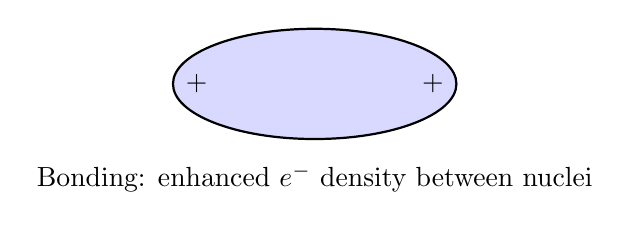
\begin{tikzpicture}
  % Bonding diagram
  \node at (0,0) {$+$};
  \node at (3,0) {$+$};
  % Electron cloud between nuclei
  \draw[thick, fill=blue!15] (1.5,0) ellipse (1.8cm and 0.7cm);
  \node at (0,0) {$+$};
  \node at (3,0) {$+$};
  \node at (1.5, -1.2) {Bonding: enhanced $e^-$ density between nuclei};
\end{tikzpicture}
\end{center}

Because of the constructive interference, there is a higher probability of finding the electron between the two nuclei, which lowers the overall energy of the system and forms a stable bond.

\section*{2. Hydrogen Atom}

\textbf{(a)} The longest wavelength has least energy, which is the $E_3 \to E_2$ transition.

\[
E_3 = -1.5\ \text{eV}
\]
\[
E_2 = -3.4\ \text{eV}
\]

\[
\Delta E = E_3 - E_2 = -1.5 - (-3.4) = 1.9\ \text{eV}
\]
\[
\lambda = \frac{hc}{\Delta E} = \frac{1241\ \text{eV}\cdot\text{nm}}{1.9\ \text{eV}} \approx \boxed{653\ \text{nm (a red wavelength)}}
\]

\textbf{(b)}
\[
E_1 = -13.6\ \text{eV}
\]
\[
E_5 = -0.54\ \text{eV}
\]
\[
\Delta E = E_5 - E_1 = -0.54 - (-13.6) = \boxed{13.06\ \text{eV}}
\]

\textbf{(c)}
\[
\frac{P(E_5)}{P(E_1)} = e^{-\Delta E / k_B T} = \frac{1}{1000}
\]
\[
-\frac{13.056}{k_B T} = \ln(\frac{1}{1000}) = -6.908
\]
\[
k_B T = \frac{13.056}{6.908} = 1.890 \text{ eV}
\]
\[
T = \frac{1.890 \text{ eV}}{8.617 \times 10^{-5} \text{ eV/K}} = \boxed{21{,}900 \text{ K}}
\]

\section*{3. Chemical Reactions}

\textbf{(a)} The three standing waves on the double-well potential:

\begin{center}
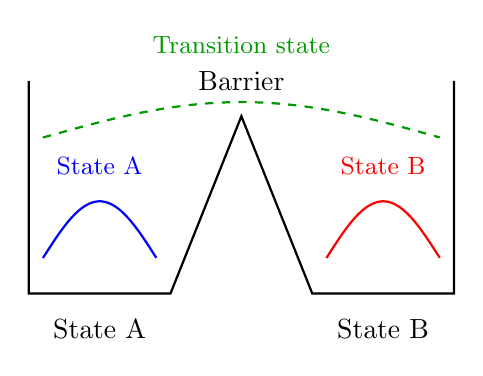
\begin{tikzpicture}[scale=0.9]
  % Double well potential
  \draw[thick] (0,3) -- (0,0) -- (2,0) -- (3,2.5) -- (4,0) -- (6,0) -- (6,3);
  \node at (1, -0.5) {State A};
  \node at (5, -0.5) {State B};
  \node at (3, 3) {Barrier};

  % State A wave (localized in left well)
  \draw[blue, thick, domain=0.2:1.8, samples=50] plot (\x, {0.8*sin(deg(3.14*(\x-0.2)/1.6)) + 0.5});
  \node[blue] at (1, 1.8) {\small State A};

  % State B wave (localized in right well)
  \draw[red, thick, domain=4.2:5.8, samples=50] plot (\x, {0.8*sin(deg(3.14*(\x-4.2)/1.6)) + 0.5});
  \node[red] at (5, 1.8) {\small State B};

  % Transition state (spread across both wells)
  \draw[green!60!black, thick, dashed, domain=0.2:5.8, samples=80] plot (\x, {0.5*sin(deg(3.14*(\x-0.2)/5.6)) + 2.2});
  \node[green!60!black] at (3, 3.5) {\small Transition state};
\end{tikzpicture}
\end{center}

The molecule must pass through the transition state because to convert from A to B, the wave must reorganize from being localized in well A to being localized in well B. This requires enough energy to exist at the top of the barrier, where the wavefunction is spread across both wells. The transition state represents the unstable intermediate configuration during bond rearrangement.

\textbf{(b)} The rate of crossing a barrier is given by:
\[
\text{rate} = \nu \, e^{-E_{\text{barrier}} / k_B T}
\]
where $\nu \approx 10^{13}$ s$^{-1}$ is the molecular vibration frequency. At body temperature ($T = 310$ K):
\[
k_B T = (8.617 \times 10^{-5})(310) = 0.02671 \text{ eV}
\]

\bigskip

\textbf{Barrier = 100 meV = 0.1 eV:}
\[
\text{rate} = 10^{13} \times e^{-0.1/0.02671} = 10^{13} \times e^{-3.74} = 10^{13} \times 0.024 = 2.4 \times 10^{11} \text{ s}^{-1}
\]
\[
\text{time} = \frac{1}{\text{rate}} \approx \boxed{4 \times 10^{-12} \text{ s (picoseconds)}}
\]

\textbf{Barrier = 1 eV:}
\[
\text{rate} = 10^{13} \times e^{-1/0.02671} = 10^{13} \times e^{-37.4} = 10^{13} \times 5.3 \times 10^{-17} = 5.3 \times 10^{-4} \text{ s}^{-1}
\]
\[
\text{time} = \frac{1}{\text{rate}} \approx \boxed{1{,}900 \text{ s} \approx 32 \text{ minutes}}
\]

\textbf{Barrier = 10 eV:}
\[
\text{rate} = 10^{13} \times e^{-10/0.02671} = 10^{13} \times e^{-374} \approx 10^{13} \times 10^{-163} = 10^{-150} \text{ s}^{-1}
\]
\[
\text{time} = \frac{1}{\text{rate}} \approx \boxed{10^{150} \text{ s (far longer than the age of the universe)}}
\]

Small barriers allow reactions to occur almost instantaneously at body temperature. Medium barriers take minutes---enzymes can lower these to speed up biological reactions. Large barriers make spontaneous reactions essentially impossible, which is why covalent bonds (like those in DNA) are stable at physiological temperatures.

\end{document}
